\documentclass[12pt]{article}
\usepackage[utf8]{inputenc}
\usepackage{graphicx}
\usepackage[letterpaper,width=150mm,top=25mm,bottom=25mm]{geometry}

\usepackage[hidelinks]{hyperref}
\usepackage{ulem}

\setlength{\parskip}{1ex}
\usepackage[spanish]{babel}

\title{
\vspace{-2cm}
{
\includegraphics[height=2.2cm]{imgs/logoUAMC.eps}}
\hspace{3.5cm}
{
\includegraphics[height=3.4cm]{imgs/logoLicTySI.eps}}\\
\vspace{1cm}
{\large Sistemas Operativos}\\
{Práctica 1. Introducción al interprete de comandos.}
}

\author{Prof. Jorge Matadamas Hernández}
\date{Octubre del 2022}

\begin{document}

\maketitle

%\begin{abstract}
%The main idea of this project is to study the ........

%\end{abstract}

\section{Objetivo}
Que el alumno practique la interacción con el sistema operativo mediante el interprete de comandos.


\section{Introducción}

\subsection{Shell}

Una de las funciones del sistema operativo consiste en ser un intermediario entre los recursos de un sistema de cómputo y los usuarios humanos. Las dos principales formas en que los usuarios pueden interactuar con el sistema operativo son: la interfaz gráfica de usuario (GUI) y la interfaz de líneas de comandos (CLI o shell). El shell predeterminado para muchas distribuciones de Linux es GNU Bourne-Again Shell (bash). Cuando una shell se utiliza de manera interactiva, muestra un \textit{shell prompt} que termina con el carácter {\ttfamily\$} o {\ttfamily\#}, dependiendo de si el usuario es un usuario convencional o el superusuario \textit{root} con mayores privilegios. 

\begin{verbatim}
Ejecutar una shell           (ambiente gráfico vs linea de comandos)
Obtener privilegios de root  (su -, sudo, sudo su, $ vs #)
Instalar vim y git           (apt-get install, gestores de paquetes)
Salir de la shell de root    (exit o ctrl+d)
\end{verbatim}



\subsection{Comandos}

La interacción se da cundo el usuario escribe un comando y el sistema operativo responde con una serie de acciones y/o resultados, según el comando. Los comandos están compuestos por tres partes:

\begin{itemize}
	\item Comando. Es el comando a ejecutar.
	\item Opciones. Permiten ajustar el comportamiento del comando.
	\item Argumentos. Generalmente son los destinos del comando.
\end{itemize} 

Las opciones, por lo general, son precedidas por uno o dos guiones ({\ttfamily -a o --all}) para que se distingan de los argumentos. Por ejemplo, el comando ''ls'' muestra los archivos y directorios del directorio actual; si adicionalmente se le agregan los modificadores ''l'' y ''a'' los muestra en forma de lista e incluye los archivos y directorios ocultos; si adicionalmente se le pasa un argumento mostrará los archivos y directorios del directorio que se le pase como argumento:

\begin{verbatim}
         ls
         ls -l -a                  (ocultos, extensiones)
         ls -la Escritorio/
\end{verbatim}	

Para conocer las opciones y los argumentos que algún comando acepta y el orden en que se espera que se introduzcan, se puede consultar el manual, ejecutando el comando {\ttfamily man} seguido del comando sobre el cuál se desea saber, por ejemplo:

\begin{verbatim}
          man ls
          man man
\end{verbatim}

Nota: Para salir del manual se presiona la tecla ''q''.

El manual, entre otras cosas, muestra una descripción del comando, la forma en que se utiliza y una lista de argumentos; usa las siguientes convenciones:

\begin{itemize}
\item Las palabras en \textbf{\texttt{negritas}} se escriben tal cual.
\item Los corchetes ''{\ttfamily [ ]}'' indican elementos opcionales.
\item Lo que va seguido de ''{\ttfamily ...}'' se puede repetir.
\item Si hay múltiples elementos separados por ''{\ttfamily |}'', únicamente se puede especificar uno de ellos.
\end{itemize}

\newpage
Ejemplos de comanods:

\begin{verbatim}
          clear            (ctrl+l)
          cd ruta          (rutas absolutas y relativas)
                           (sin ruta, ..,~,-)
          pwd
          mkdir            (-p)
          cp               (-r)
          mv               
          rm               (-r)
          touch            (extensiones, ocultos)
          
          find . -name '*.jpg'     (comodínes * y ?)
          head -n 3 /etc/passwd
          tail -n 3 /etc/passwd
          wc                       (renglones, palabras, bytes)
          wc -l /etc/passwd
          history
          vim .bash_history
          
          exit              (ctrl+d)
\end{verbatim}

Además del manual, en Internet hay mucha información sobre cómo utilizar un comando en particular o qué comando utilizar para una tarea específica.

\subsection{Estructura del sistema de archivos}

El sistema de archivos son las reglas y la forma en que el sistema operativo almacena y gestiona los archivos. La estructura de los archivos en linux es muy parecida a la que se muestra en la Figura \ref{filesystem} (falta el directorio \texttt{/var}).

\begin{figure}[!ht]
\begin{center}
    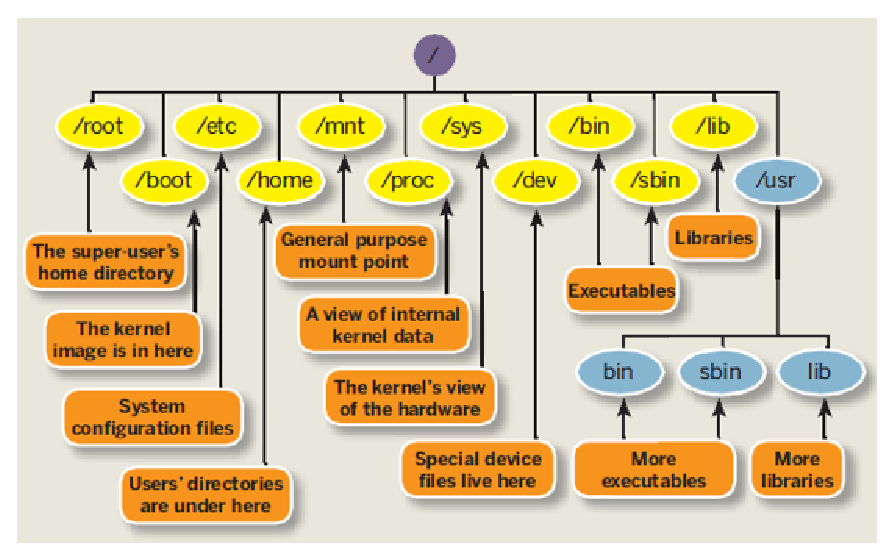
\includegraphics[width=14cm]{imgs/filesystem.eps}
	\caption{Estructura del sistema de archivos Linux.}
	\label{filesystem}    
\end{center}
\end{figure}

\subsection{Redireccionamiento}

 El redireccionamiento de E/S reemplaza los canales predeterminados (stdin, stdout, stderr) por otros archivos o dispositivos. Así es posible enviar la salida de un proceso a un archivo utilizando ''$>$'' (si el archivo existe se sobre escribe) y ''$>$ $>$'' (si el archivo existe se agrega al final). 
\begin{verbatim}
          date > fecha.txt
          cat fecha.txt
          date >> fecha.txt
          ls -l ~ > salida.txt
\end{verbatim}

El archivo \texttt{/dev/null} es un archivo especial que siempre está vacío, a pesar de que se escriba en él cualquier cantidad de información, por lo general se utiliza para redireccionar a él la salida estándar o el error estándar de algunos procesos, sin preocuparse por  ocupar espacio en el disco.

\begin{verbatim}
          ls -l ~ > /dev/null
\end{verbatim}

\subsection{Tuberías}

Las tuberías (pipe) nos permiten ejecutar secuencias de comandos, permiten que la salida de un comando sea la entrada de otro. Los comandos se escriben separados por ''{\ttfamily |}''.

\begin{verbatim}
          history | grep cp
          ps aux | grep bash
\end{verbatim}

\subsection{vim}

Vim es un editor de textos que funciona desde el shell, es decir que no necesita una interfaz gráfica. Se puede utilizar para editar archivos de configuración del sistema y para hacer programas o scripts. Una forma de ejecutarlo es tecleando en el shell:

\begin{verbatim}
          vim nombredelarchivo
\end{verbatim}	

Donde ''{\ttfamily nombredelarchivo}'' es el nombre de un archivo, si el archivo no existe se crea. 
 
Cuando vim arranca lo hace en modo ''comando'', desde el modo ''comando'' se puede cambiar al modo ''edición'' prsionando la tecla ''i'' o al modo ''comando extendido'' presionando la tecla '':''. Para regresar al modo ''comando'' se presiona la tecla ''esc''. 

En el modo ''comando'' se pueden teclear comandos para navegar el archivo. En el modo ''edición'' se pueden utilizar las teclas: flechas, enter, backspace, shift, letras y números para navegar y editar el archivo. Mientras que en el modo ''comando extendido'' se pueden teclear comandos para hacer búsquedas, editar y guardar el archivo (entre otros).

El flujo básico de trabajo es:

\begin{itemize}
\item Abrir un archivo con:  {\ttfamily vim nombredelarchivo}
\item Presionar {\ttfamily i} para entrar al modo edición
\item Editar el archivo
\item Presionar {\ttfamily esc} para vlolver al modo comando
\item Escribir {\ttfamily :w} para guardar los cambios
\item O escribir {\ttfamily :wq} para guardar y salir vim
\item O escribir {\ttfamily :q!} para descartar los últimos cambios y salir 
\end{itemize}   

Ejemplos:
\begin{verbatim}
          vim hola.txt     (se crea y se edita)
          cat hola.txt     (se revisa su contenido)
          
          vim hola.c       (escribir un hola mundo en C)
          gcc hola.c       (compilación, opción -o)
          ./a.out          (ejecución)
          
          vim Hola.java    (escribir un hola mundo en Java)
          javac Hola.java  (compilación, .class, bytecode/JVM)
          java Hola        (ejecución)
\end{verbatim}

\subsection{Scripts bash}
Un \textit{script bash} es un archivo de texto con comandos bash, los cuales serán ejecutados en el shell sin tener que teclearlos uno a uno. Es costumbre que el archivo tenga la extensión {\ttfamily .sh} y que la primera linea sea el siguiente comentario:

\begin{verbatim}
          #!/bin/bash          (ruta donde se encuentra bash)
\end{verbatim}

El script se ejecuta escribiendo en el shell:

\begin{verbatim}
          bash nombreArchivo.sh
\end{verbatim}
o
\begin{verbatim}
          ./nombreArchivo.sh
\end{verbatim}

En el segundo caso es necesario que el archivo tenga permisos de ejecución ({\ttfamily chmod +x nombreArchivo.sh}).\\


Ejemplos de programas bash.
\begin{verbatim}
********************************
#!/bin/bash

for i in {1..10}
do
    echo Hola Mundo $i
done


********************************
#!/bin/bash

n=1
while [ $n -le 6 ]
do
  echo $n
  n=$(( $n + 1 ))
done

********************************
#!/bin/bash

echo -n "Enter Number: "
read x

if [ $((x%2)) == 0 ]; then
  echo "Number is Even"
else
  echo "Number is Odd"
fi

********************************
#!/bin/bash

if [ "$1" = "" ]
then
        echo "Debe indicar el nombre del directorio a utilizar."
        exit
fi

if [ -e $1 ]
then
        echo "OK: existe el directorio"
else
        mkdir $1
        echo "Creando el directorio: " $1
fi

echo "Accediendo al directorio..."
cd $1

dir="https://www.debian.org/logos/openlogo-nd-100.jpg"

wget -q $dir

if [ $? -ne 0 ]
then
        echo "Archivo no descargado: Error "
else
        echo "Archivo descargado: OK"
fi
********************************
\end{verbatim}

Referencia Bash scritping: \url{https://devhints.io/bash}


\subsection{awk}

El comando awk (que también es un lenguaje) es útil para procesar y analizar texto que está organizado en líneas y columnas, se utiliza en los \textit{scripts} para filtrar los resultados de otros comandos y el contenido de archivos. La forma básica de un comando awk es: 

\begin{verbatim}
          awk [condición] '{comandos}' archivo
\end{verbatim}

Ejemplos de uso de \texttt{awk}

\begin{verbatim}
awk -F : '{print $1}' /etc/passwd

Imprime la primera columna del archivo /etc/passwd considerando que el carácter 
de separación es ":"


ps -eo pid,user,comm | grep "bash" | head -n 1 | awk '{print $1}'

¿Que significa el resultado y cómo se obtiene?
comandos utilizados: ps, grep, head, awk

\end{verbatim}








\section{Actividades}
Conteste brevemente las siguientes preguntas:
\begin{enumerate}
    \item ¿Qué es un sistema operativo?
    \item ¿Qué es un intérprete de comandos?
    \item ¿Cómo se llama el shell por defecto de Ubuntu, Red-hat, MacOS y Windows?
    \item ¿Además de bash qué otros shell existen?
    \item ¿Qué es un gestor de paquetes? y ¿Cuál es el nombre del gestor de paquetes por defecto de Ubunto y de Fedora?
    \item ¿Cual es la relación entre Debian y Ubunto? y entre ¿Red-Hat y Fedora?
    \item ¿Qué información se guarda en el directorio \texttt{/var}?
    \item Investigue para que sirven los siguientes comandos: {\ttfamily whoami, grep, less, more, uname, top, du, df, ps, kill, find, chmod, chown, ssh, scp, uptime, w, wget, curl, mount, tree}
    \item Resuelva los siguientes problemas haciendo un \textit{script bash} con los comandos y tuberías necesarias (Incluir en la práctica la captura de pantalla de cada código y sus resultados).

	\begin{itemize}
		\item obtener una lista de todos los procesos de tu usuario
		\item Mostrar la cantidad de procesadores y cores que tiene la computadora.
		\item Mostrar la cantidad de memoria (en GBytes) que tiene la computadora.
		\item Mostrar el número de procesos que se están ejecutando en el sistema.
		\item Mostrar cuantos procesos corresponden al usuario root y cuantos a su usuario.
		\item Mostrar la información (idUsuario, nombre, \% de consumo de CPU) de los 3 procesos que consumen más CPU.
		\item Validar si una contraseña tiene un buen formato: mínimo 8 caracteres, al menos un símbolo numérico, al menos uno de los siguientes símbolos: {\ttfamily @, \#, \$, \%, \&, *, +, -, =}
		
	\end{itemize}
\end{enumerate}

%\section {References}
%\bibliographystyle{IEEEtranS}
%\bibliography{refs}

\end{document}
